\documentclass[11pt,a4paper]{article}

% ---- Packages ----------------------------------------------------------
\usepackage[utf8]{inputenc}
\usepackage[T1]{fontenc}
\usepackage{lmodern}
\usepackage[margin=1in]{geometry}
\usepackage{microtype}
\usepackage{amsmath}
\usepackage{amssymb}
\usepackage{titlesec}
\usepackage{enumitem}
\usepackage{booktabs}
\usepackage{array}
\usepackage{tabularx}
\usepackage{xcolor}
\usepackage{graphicx}
\usepackage{fancyhdr}
\usepackage{tikz}
\usetikzlibrary{positioning, arrows.meta, shapes.geometric, fit, calc, backgrounds, decorations.pathreplacing}
\usepackage[hidelinks,colorlinks=true,linkcolor=black,citecolor=teal,urlcolor=teal]{hyperref}
\usepackage{parskip}
\usepackage{float}

% ---- Color palette (deliberately different from v1) --------------------
\definecolor{accent}{HTML}{0F766E}
\definecolor{accentlight}{HTML}{CCFBF1}
\definecolor{warm}{HTML}{B45309}
\definecolor{warmlight}{HTML}{FEF3C7}
\definecolor{cool}{HTML}{1E3A8A}
\definecolor{coollight}{HTML}{DBEAFE}
\definecolor{neutral}{HTML}{475569}
\definecolor{neutrallight}{HTML}{F1F5F9}

% ---- TikZ styles -------------------------------------------------------
\tikzset{
  data/.style    = {rectangle, rounded corners=3pt, draw=neutral, thick,
                    fill=neutrallight, minimum width=2.4cm, minimum height=0.85cm,
                    align=center, font=\small},
  proc/.style    = {rectangle, rounded corners=3pt, draw=cool, thick,
                    fill=coollight, minimum width=2.4cm, minimum height=0.85cm,
                    align=center, font=\small},
  model/.style   = {rectangle, rounded corners=3pt, draw=accent, very thick,
                    fill=accentlight, minimum width=3.0cm, minimum height=1.0cm,
                    align=center, font=\small},
  artifact/.style= {rectangle, rounded corners=3pt, draw=warm, thick,
                    fill=warmlight, minimum width=2.4cm, minimum height=0.85cm,
                    align=center, font=\small},
  device/.style  = {rectangle, rounded corners=3pt, draw=neutral, thick,
                    fill=neutrallight, minimum width=2.0cm, minimum height=0.7cm,
                    align=center, font=\small},
  alert/.style   = {rectangle, rounded corners=3pt, draw=red!60!black, thick,
                    fill=red!8, minimum width=2.4cm, minimum height=0.85cm,
                    align=center, font=\small},
  pkt/.style     = {rectangle, draw=cool!70, thick, fill=coollight,
                    minimum width=0.55cm, minimum height=0.55cm,
                    inner sep=1pt, font=\tiny},
  feat/.style    = {circle, draw=accent!70, thick, fill=accentlight,
                    inner sep=1pt, minimum size=0.45cm, font=\tiny},
  fuse/.style    = {diamond, draw=warm, thick, fill=warmlight,
                    aspect=2, inner sep=1pt, align=center, font=\small},
  arr/.style     = {-{Latex[length=2mm,width=1.6mm]}, thick, draw=neutral!80},
  darr/.style    = {-{Latex[length=2mm,width=1.6mm]}, thick, draw=neutral!80, dashed},
}

% ---- Header / Footer ---------------------------------------------------
\pagestyle{fancy}
\fancyhf{}
\fancyhead[L]{\small Flow-Pattern Anomaly Detection at the IoT Gateway}
\fancyhead[R]{\small Madhav Dogra --- DRDO Proposal}
\fancyfoot[C]{\thepage}
\renewcommand{\headrulewidth}{0.4pt}

% ---- Section formatting ------------------------------------------------
\titleformat{\section}{\normalfont\Large\bfseries\color{cool}}{\thesection}{0.7em}{}
\titleformat{\subsection}{\normalfont\large\bfseries\color{neutral!80!black}}{\thesubsection}{0.6em}{}

% ---- Title page info ---------------------------------------------------
\title{\textbf{Flow-Pattern Anomaly Detection at the IoT Gateway} \\[0.5em]
       \large A Pre-trained Mamba Approach \\[0.3em]
       \normalsize DRDO Internship Proposal}
\author{Madhav Dogra}
\date{\today}

% =======================================================================
\begin{document}
\maketitle
\thispagestyle{empty}

% ---- Abstract ----------------------------------------------------------
\begin{abstract}
\noindent
We propose an anomaly detector for the \textbf{smart-home IoT} traffic path (cameras, sensors, smart bulbs, voice assistants, and similar consumer devices) that is deployable at the home gateway, works on encrypted traffic, and detects both known attacks and zero-day flows. The detector is built on three architectural commitments that distinguish it from conventional IoT IDS work. \textbf{First}, each flow is represented as an ordered sequence of per-packet features --- a \emph{flow pattern} --- rather than as an aggregated statistic vector. \textbf{Second}, a Mamba selective state-space-model encoder is pre-trained self-supervised on unlabelled benign traffic, producing a representation that is then shared by all downstream tasks. \textbf{Third}, the backbone is a state-space model rather than a transformer, on the grounds that recent work (NetMamba) has demonstrated comparable accuracy to BERT-class encrypted-traffic models such as ET-BERT at a fraction of the parameter and latency cost. Two downstream heads consume the encoder: a supervised softmax classifier for the seven CICIoT2023 attack categories and a one-class anomaly scorer for zero-day detection. The system is evaluated on CICIoT2023 (primary), TON\_IoT (cross-dataset generalisation), and IoT-23 (real-world malware). SHAP attributions, an FGSM adversarial-robustness study, and a post-quantisation latency / memory benchmark on gateway-class hardware complete the deliverable. The 12-week plan culminates in a reproducible code repository, a pre-trained encoder checkpoint, a benchmark table, and a written report.
\end{abstract}

% =======================================================================
\section{Background and Motivation}

\subsection{Why smart-home IoT is the soft layer of modern networks}
The detector targets the class of devices typically found in a \textbf{smart home}: IP cameras, environmental and motion sensors, smart bulbs, voice assistants, thermostats, doorbells, smart plugs, and the home gateway / router itself. These devices are now the most exposed and least defended surface in most networks. They ship with weak default credentials, run firmware that is rarely patched, frequently have physical-access exposure, and lack the compute headroom for endpoint-resident security tooling. The Mirai botnet, built almost entirely from compromised IP cameras and home routers, is the canonical demonstration that this surface is exploitable at scale. CICIoT2023's 105-device testbed is dominated by exactly this class of consumer IoT, which makes it the right training corpus.

\subsection{Why detect at the gateway, not at the device}
Endpoint-resident agents are not an option for most IoT devices, so detection must happen on the network path. Within that path, the IoT gateway is the natural choke point: every device flow passes through it on its way to the central collector, and the gateway is the only place where the operator can deploy modern compute without instrumenting every device. We therefore target the gateway as the deployment environment. This commits us to a tight latency and memory budget --- gateway hardware is typically Raspberry-Pi-class --- but gives us full visibility over the upstream traffic.

\subsection{Why flow patterns, not aggregated statistics}
Conventional IoT IDS work aggregates each flow into a fixed-size vector of summary statistics --- mean packet length, total bytes, IAT standard deviation, flag counts, and so on. This representation is convenient but lossy: it is permutation-invariant by construction, so the temporal structure of a flow is discarded. Yet many attack signatures \emph{live} in the temporal structure: beaconing patterns, scan progressions, handshake oddities, burst behaviour. The alternative is to keep the flow as a sequence --- the ordered per-packet feature vectors of (say) the first 32 packets of the connection --- and let a sequence model do the aggregation implicitly through learning. We adopt this representation.

\subsection{Why a state-space model, not a transformer}
The reference architecture for pre-trained encrypted-traffic representations is ET-BERT~\cite{ETBERT}, a BERT-base-scale masked-language-model trained on raw datagram bytes. ET-BERT achieves state-of-the-art accuracy on multiple encrypted-traffic classification benchmarks, but at $\approx$110\,M parameters it is structurally incompatible with gateway-class hardware. The selective state-space model family (S4D~\cite{S4D}, Mamba~\cite{Mamba}, Mamba-2~\cite{SSD}) gives us a way around this constraint: linear-time inference in sequence length, transformer-comparable quality on long-sequence tasks, and substantially lower parameter counts at comparable accuracy. NetMamba~\cite{NetMamba} applies exactly this idea to network traffic classification, reporting ET-BERT-class accuracy at a fraction of the cost. We adopt the NetMamba design philosophy as the core of our detector.

\subsection{Four pillars of the proposed design}
The proposal sits on four explicit design commitments:
\begin{enumerate}[leftmargin=*, itemsep=2pt]
  \item \textbf{Flow patterns}, not aggregated statistics, as the input representation.
  \item \textbf{Self-supervised pre-training} of a shared encoder on benign-only traffic, before any supervised signal is applied.
  \item \textbf{A Mamba backbone}, chosen for the cost-quality trade-off on long-sequence input at edge scale.
  \item \textbf{Analyst-facing evaluation}: SHAP attributions on every alert, plus an FGSM adversarial stress test, on top of standard classification metrics.
\end{enumerate}

% =======================================================================
\section{Related Work and Architectural Choices}

\subsection{Pre-trained representations for network traffic}
\textbf{ET-BERT}~\cite{ETBERT} (Lin~et~al., WWW 2022) is the reference architecture for the pre-train-then-fine-tune paradigm on network traffic. It tokenises raw datagram bytes, pre-trains a BERT-base transformer with masked-token and same-origin-sentence objectives, and fine-tunes on downstream classification. It defines the paradigm we follow. Its cost is the reason we do not use it directly.

\textbf{NetMamba}~\cite{NetMamba} (Wang~et~al., 2024) is the closest precedent to our work. It replaces ET-BERT's transformer with a unidirectional Mamba, pre-trains on packet-byte sequences, and reports accuracy competitive with ET-BERT at substantially lower parameter count and inference latency. We use NetMamba as the architectural template for the encoder.

\textbf{ET-SSL}~\cite{ETSSL} establishes that self-supervised contrastive learning over flow-statistic views of encrypted traffic produces representations transferable to anomaly detection. It motivates an optional contrastive variant of our pre-training objective.

\subsection{The state-space-model line}
\textbf{S4D}~\cite{S4D} (Gu, Goel, R\'e, NeurIPS 2022) is the diagonal parameterisation of structured state-space models. It is the practical, easy-to-train form of S4 on which all subsequent work in this family builds. Foundational reading.

\textbf{Mamba}~\cite{Mamba} (Gu \& Dao, 2023) introduces \emph{selective} state-space models: the state-transition matrix becomes input-dependent, which gives the model the capacity to selectively retain or discard information along the sequence. The result is linear-time inference in sequence length with transformer-comparable quality. Our encoder uses Mamba blocks.

\textbf{Mamba-2 / Structured State Space Duality (SSD)}~\cite{SSD} (Dao \& Gu, ICML 2024) shows that transformers and SSMs are two views of a single underlying structure, yielding a faster and more expressive successor to Mamba. Reserved as a stretch-goal swap.

\subsection{IoT IDS datasets, benchmarks, and surveys}
The current default benchmark is \textbf{CICIoT2023}~\cite{CICIoT2023} (Neto et al., 2023), a real-device capture of 105 devices and 33 attack types across 7 categories. \textbf{TON\_IoT} is widely used as a cross-dataset generalisation target. \textbf{IoT-23} (Stratosphere Lab) contains real-world malware captures including Mirai, Torii, and Okiru. Background context is set by the comprehensive review of Morshedi et al.~\cite{Morshedi2025} and the MDPI survey~\cite{Sensors2023}. The transformer-cost-on-gateway argument is empirically grounded in the Nature \emph{Sci.\ Rep.} study~\cite{TransformerIoT}, which directly motivates our move to SSMs.

\subsection{Explainability and adversarial robustness}
We adopt SHAP~\cite{XAI} as the per-alert explanation mechanism --- the analyst-facing standard for IDS literature. For adversarial evaluation we follow the recent IoT-IDS adversarial-robustness study~\cite{AdvIoT}, which uses FGSM as the entry-point benchmark and shows that SHAP DeepExplainer attribution fingerprints separate clean and adversarial inputs --- a useful secondary signal.

\subsection{Stretch-goal references}
For the optional graph-aware extension we follow E-GraphSAGE~\cite{EGraphSAGE} (Lo et al.). For federated training across DRDO sensor sites that cannot share raw pcaps we draw on the hybrid DL+FL IDS work~\cite{FLIDS} and PEIoT-DS~\cite{PEIoTDS}.

% =======================================================================
\section{Proposed System}

\subsection{At a glance}
A flow arriving at the IoT gateway is reduced to a fixed-length sequence of per-packet feature vectors --- the flow pattern. This sequence is encoded by a Mamba network whose weights have been pre-trained self-supervised on a large set of benign flows. The resulting embedding is read by two downstream heads in parallel: a supervised classifier for known attack categories and a one-class anomaly scorer for zero-day detection. A rule-based fusion gate raises an alert if either head exceeds threshold; SHAP attributions over the input sequence are attached to every alert before it is forwarded to the SOC over Kafka. The deployment context is shown in Figure~\ref{fig:context}.

% ---- Figure 1: Deployment context (compact) ----------------------------
\begin{figure}[H]
\centering
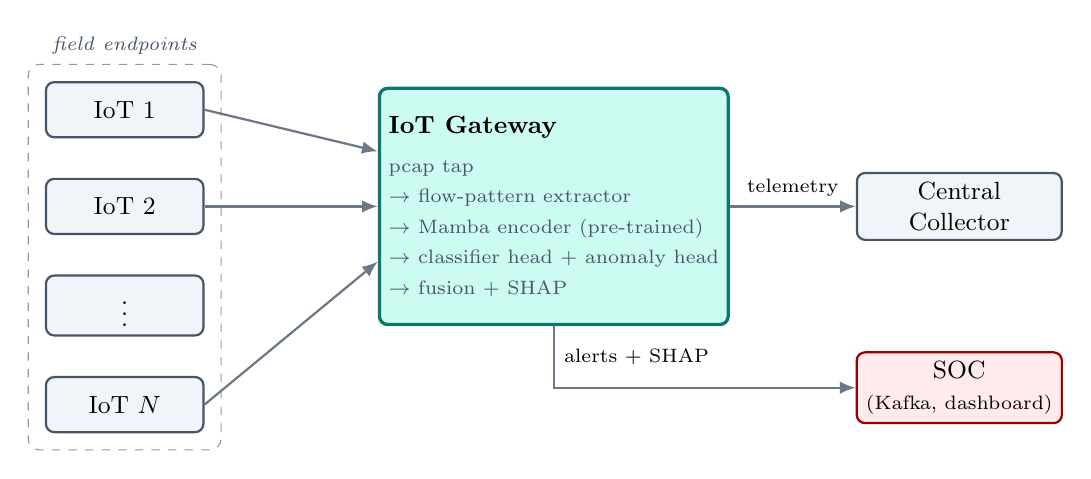
\begin{tikzpicture}[node distance=0.5cm and 1.4cm]

  \node[device]                  (d1) {IoT 1};
  \node[device, below=of d1]     (d2) {IoT 2};
  \node[device, below=of d2]     (d3) {\vdots};
  \node[device, below=of d3]     (dn) {IoT $N$};

  \node[draw=neutral!60, dashed, rounded corners, fit=(d1)(dn), inner sep=6pt,
        label={[font=\scriptsize\itshape, neutral]above:field endpoints}] (grp) {};

  \node[model, right=2.2cm of d2, minimum width=4.4cm, minimum height=3.0cm,
        align=left] (gw) {\textbf{IoT Gateway}\\[3pt]
        \scriptsize\textcolor{neutral}{pcap tap}\\
        \scriptsize\textcolor{neutral}{$\to$ flow-pattern extractor}\\
        \scriptsize\textcolor{neutral}{$\to$ Mamba encoder (pre-trained)}\\
        \scriptsize\textcolor{neutral}{$\to$ classifier head + anomaly head}\\
        \scriptsize\textcolor{neutral}{$\to$ fusion + SHAP}};

  \node[data, right=1.6cm of gw, minimum width=2.6cm] (cc) {Central \\ Collector};
  \node[alert, below=1.4cm of cc, minimum width=2.6cm] (soc) {SOC \\ \scriptsize (Kafka, dashboard)};

  \draw[arr] (d1.east) -- ([yshift=0.7cm]gw.west);
  \draw[arr] (d2.east) -- (gw.west);
  \draw[arr] (dn.east) -- ([yshift=-0.7cm]gw.west);
  \draw[arr] (gw.east) -- node[above, font=\scriptsize]{telemetry} (cc.west);
  \draw[arr] (gw.south) |- node[pos=0.25, right, font=\scriptsize]{alerts + SHAP} (soc.west);

\end{tikzpicture}
\caption{Deployment context. The detector is contained entirely within the IoT gateway, the natural choke point on the upstream path. Telemetry continues to the central collector unmodified; alerts and SHAP attributions are forwarded out-of-band to the SOC. The detector does not gate telemetry delivery.}
\label{fig:context}
\end{figure}

\subsection{Flow-pattern representation}
For each bidirectional flow we extract its first $K$ packets ($K \approx 32$, ablated). Each packet is reduced to a fixed-dimensional feature vector $p_t \in \mathbb{R}^d$ comprising:
\begin{itemize}[leftmargin=*, itemsep=1pt]
  \item Packet length and direction (uplink vs.\ downlink).
  \item Inter-arrival time since the previous packet of this flow.
  \item TCP flag bits (SYN, ACK, FIN, RST, PSH, URG).
  \item Selected IP / TCP header-level fields (TTL, window size, header length).
  \item Optionally the first $M$ bytes of the packet (per ET-BERT and NetMamba). These bytes are treated as an opaque pattern; the model never parses payload semantics, so the approach remains valid on encrypted traffic.
\end{itemize}

The flow is then the length-$K$ sequence $\mathbf{x} = (p_1, p_2, \ldots, p_K)$. This contrasts deliberately with the conventional aggregated representation, as shown in Figure~\ref{fig:representation}: the aggregated vector is permutation-invariant and discards order, while the sequence preserves the temporal structure that the downstream sequence model can exploit.

% ---- Figure 2: Representation contrast (stacked vertically) -----------
\begin{figure}[H]
\centering
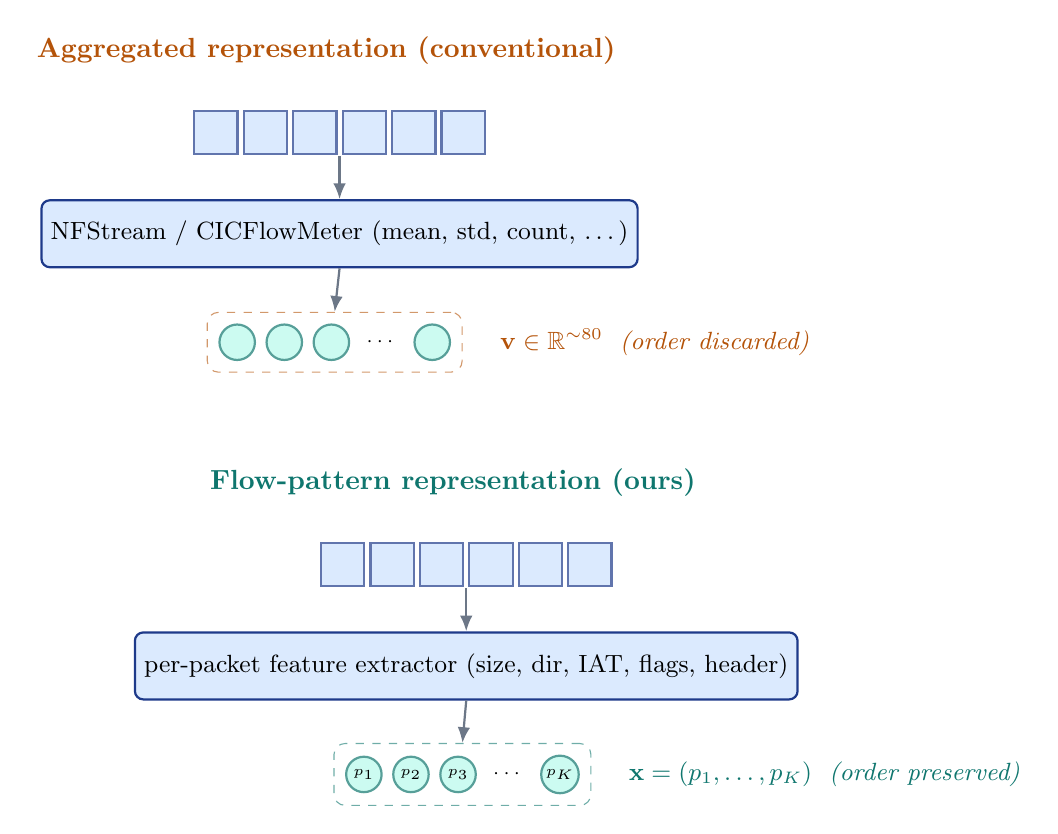
\begin{tikzpicture}[node distance=0.45cm and 0.9cm]

  % ----- TOP: Aggregated representation -----
  \node[font=\bfseries, color=warm] (lhd) {Aggregated representation (conventional)};

  \node[pkt, below=0.45cm of lhd, xshift=-1.4cm] (lp1) {};
  \node[pkt, right=0.05cm of lp1] (lp2) {};
  \node[pkt, right=0.05cm of lp2] (lp3) {};
  \node[pkt, right=0.05cm of lp3] (lp4) {};
  \node[pkt, right=0.05cm of lp4] (lp5) {};
  \node[pkt, right=0.05cm of lp5] (lp6) {};
  \node[fit=(lp1)(lp6), inner sep=0pt] (lpkts) {};

  \node[proc, below=0.55cm of lpkts, minimum width=5.6cm] (lagg)
       {\small NFStream / CICFlowMeter (mean, std, count, \ldots)};

  \node[feat, below=0.7cm of lagg, xshift=-1.3cm] (lf1) {};
  \node[feat, right=0.12cm of lf1] (lf2) {};
  \node[feat, right=0.12cm of lf2] (lf3) {};
  \node[right=0.08cm of lf3, font=\scriptsize] (ldots) {$\cdots$};
  \node[feat, right=0.08cm of ldots] (lf4) {};

  \node[draw=warm!60, dashed, rounded corners, fit=(lf1)(lf4), inner sep=4pt] (lvec) {};
  \node[right=0.35cm of lvec, font=\small, color=warm] (lvlab)
       {$\mathbf{v}\in\mathbb{R}^{\sim 80}$~~\emph{(order discarded)}};

  \draw[arr] (lpkts.south) -- (lagg.north);
  \draw[arr] (lagg.south) -- (lvec.north);

  % ----- BOTTOM: Flow-pattern representation -----
  \node[font=\bfseries, color=accent, below=1.1cm of lvec, xshift=1.5cm] (rhd)
       {Flow-pattern representation (ours)};

  \node[pkt, below=0.45cm of rhd, xshift=-1.4cm] (rp1) {};
  \node[pkt, right=0.05cm of rp1] (rp2) {};
  \node[pkt, right=0.05cm of rp2] (rp3) {};
  \node[pkt, right=0.05cm of rp3] (rp4) {};
  \node[pkt, right=0.05cm of rp4] (rp5) {};
  \node[pkt, right=0.05cm of rp5] (rp6) {};
  \node[fit=(rp1)(rp6), inner sep=0pt] (rpkts) {};

  \node[proc, below=0.55cm of rpkts, minimum width=5.6cm] (ragg)
       {\small per-packet feature extractor (size, dir, IAT, flags, header)};

  \node[feat, below=0.7cm of ragg, xshift=-1.3cm] (rf1) {$p_1$};
  \node[feat, right=0.12cm of rf1] (rf2) {$p_2$};
  \node[feat, right=0.12cm of rf2] (rf3) {$p_3$};
  \node[right=0.08cm of rf3, font=\scriptsize] (rdots) {$\cdots$};
  \node[feat, right=0.08cm of rdots] (rf4) {$p_K$};

  \node[draw=accent!60, dashed, rounded corners, fit=(rf1)(rf4), inner sep=4pt] (rvec) {};
  \node[right=0.35cm of rvec, font=\small, color=accent] (rvlab)
       {$\mathbf{x}=(p_1,\ldots,p_K)$~~\emph{(order preserved)}};

  \draw[arr] (rpkts.south) -- (ragg.north);
  \draw[arr] (ragg.south) -- (rvec.north);

\end{tikzpicture}
\caption{The two input representations. The conventional aggregated vector (top) collapses an entire flow into $\approx$80 summary statistics and is invariant to packet ordering --- temporal patterns are erased before the model ever sees them. The flow-pattern representation (bottom) preserves the ordered per-packet features as a sequence, letting a sequence model learn temporal structure such as beaconing intervals, scan progressions, and burst behaviour. This is the input shift the proposal commits to.}
\label{fig:representation}
\end{figure}

\subsection{The Mamba encoder}
The encoder is a stack of Mamba blocks operating over the length-$K$ sequence. We start from a small configuration (4--6 blocks, hidden dimension 128) and adjust based on gateway-hardware ablation. A learned positional embedding is added to the per-packet features before the first block. The encoder produces a sequence of hidden states $(h_1, \ldots, h_K)$; we use the final hidden state $\mathbf{z} = h_K$ as the flow-level representation, with mean-pooling as an alternative. The encoder is the only component shared between supervised and anomaly tasks --- by design, both heads operate on the same $\mathbf{z}$.

\subsection{Downstream heads}
\textbf{Classification head.} A two-layer MLP on top of $\mathbf{z}$, followed by softmax over the seven CICIoT2023 attack categories (DDoS, DoS, Recon, Web, Brute Force, Spoofing, Mirai). Trained with focal loss ($\gamma\!\approx\!2$) to compensate for heavy class imbalance.

\textbf{Anomaly head.} A one-class scorer fitted on benign embeddings. Crucially, the anomaly head does \emph{not} consume the encoder output $\mathbf{z}$ directly: we first apply a learnable \textbf{projection MLP} $g_\phi : \mathbf{z} \mapsto \mathbf{z}_\text{ano}$ that compresses to a substantially lower-dimensional anomaly space (e.g., $\mathbb{R}^{128} \to \mathbb{R}^{32}$). One-class methods like deep SVDD are sensitive to the curse of dimensionality --- in high dimensions, distances concentrate and lose discriminative power --- so projecting down sharpens the score. The projection is trained jointly with the deep SVDD objective on benign embeddings. We default to deep SVDD (a learned hypersphere around the benign-embedding centroid) over $\mathbf{z}_\text{ano}$; Mahalanobis distance to the benign mean (also in the projected space) is the fallback. Threshold is calibrated on a held-out benign set at the 99th percentile (target 1\% FPR).

\textbf{Fusion.} An alert is raised if $s_{\text{cls}} \ge \tau_{\text{cls}}$ for any attack class \emph{or} $s_{\text{ano}} \ge \tau_{\text{ano}}$. The two thresholds are calibrated independently. A learned fusion is deferred to future work.

\subsection{Inference path}
Figure~\ref{fig:inference} shows a flow's full path through the deployed detector. The path is single-pass: each flow is encoded once, both heads consume the same embedding (with a learned projection in front of the anomaly head), and only flagged flows pay the cost of SHAP attribution. SHAP is computed over the input sequence with DeepExplainer, producing per-packet-position attributions that an analyst can read directly (\emph{e.g.}, ``flagged because of unusual IAT pattern in packets 4--7'').

\subsection{Two operating modes --- default and strong}
The gateway runs in one of two configurations, and the choice is an \textbf{operator-level setting} flipped by the admin, not a per-flow decision. One mode runs continuously by default; the other is switched on when the situation calls for it.
\begin{itemize}[leftmargin=*, itemsep=2pt]
  \item \textbf{Default mode --- low power, always on.} Smaller Mamba configuration, smaller $K$ (e.g., $K=8$), only the anomaly head active, no SHAP. This is the baseline operating point: detection is on, the compute cost is small enough for continuous use on Raspberry-Pi-class hardware, and the system catches both known and novel attacks via the anomaly score alone. Target $<2$\,ms per flow.
  \item \textbf{Strong mode --- admin-switched, full pipeline.} Full Mamba configuration, $K=32$, both classifier and anomaly heads (the latter via the projection MLP), plus SHAP attribution on every alert. Activated by the admin when needed --- elevated threat level, active incident investigation, high-value time window, or simply when the operator wants the maximum detection fidelity. Target $<10$\,ms per flow.
\end{itemize}
Switching is a configuration change applied to the gateway, not a per-flow decision and not an escalation. The same model artifacts --- encoder $\theta_*$, classifier head, projection, anomaly head --- are used in both modes; what differs is which components are engaged and at what size. Both modes produce alerts that go to the SOC. Strong mode additionally produces per-packet SHAP attributions for every alert.

% ---- Figure 3: Inference pipeline (horizontal then drop to alert) -----
\begin{figure}[H]
\centering
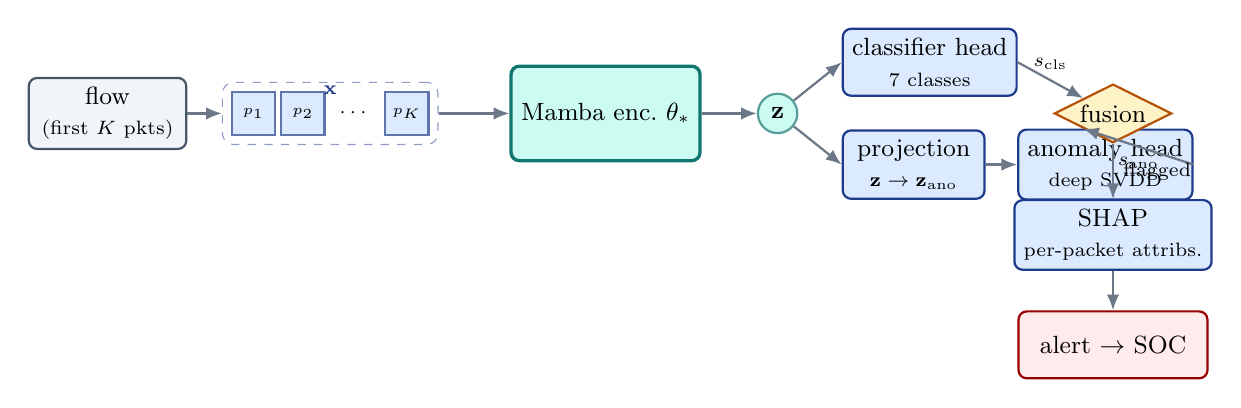
\begin{tikzpicture}[node distance=0.55cm and 0.65cm]

  % Row: input → sequence → encoder → z → heads → fusion
  \node[data, minimum width=2.0cm] (raw) {flow \\ \scriptsize (first $K$ pkts)};

  \node[pkt, right=0.55cm of raw] (p1) {$p_1$};
  \node[pkt, right=0.05cm of p1] (p2) {$p_2$};
  \node[right=0.05cm of p2, font=\scriptsize] (pdots) {$\cdots$};
  \node[pkt, right=0.05cm of pdots] (pk) {$p_K$};
  \node[draw=cool!50, dashed, rounded corners, fit=(p1)(pk), inner sep=3pt,
        label={[font=\scriptsize, below=-2pt, cool]:$\mathbf{x}$}] (seq) {};

  \node[model, right=0.9cm of seq, minimum width=2.4cm, minimum height=1.2cm] (enc)
       {Mamba enc.\ $\theta_*$};

  \node[feat, right=0.7cm of enc, minimum size=0.5cm, font=\small] (z) {$\mathbf{z}$};

  \node[proc, right=0.55cm of z, yshift=0.65cm, minimum width=2.2cm] (cls)
       {classifier head \\ \scriptsize 7 classes};
  \node[proc, right=0.55cm of z, yshift=-0.65cm, minimum width=1.8cm] (proj)
       {projection \\ \scriptsize $\mathbf{z}\to\mathbf{z}_\text{ano}$};
  \node[proc, right=0.4cm of proj, minimum width=2.0cm] (ano)
       {anomaly head \\ \scriptsize deep SVDD};

  \node[fuse, right=0.45cm of cls, yshift=-0.65cm] (fuse) {fusion};

  % Drop down: SHAP and alert below fusion
  \node[proc, below=0.7cm of fuse, minimum width=2.4cm] (shap)
       {SHAP \\ \scriptsize per-packet attribs.};
  \node[alert, below=0.5cm of shap, minimum width=2.4cm] (out)
       {alert $\to$ SOC};

  % Arrows
  \draw[arr] (raw) -- (seq);
  \draw[arr] (seq) -- (enc);
  \draw[arr] (enc) -- (z);
  \draw[arr] (z) -- (cls.west);
  \draw[arr] (z) -- (proj.west);
  \draw[arr] (proj) -- (ano);
  \draw[arr] (cls.east) -- node[above, font=\scriptsize]{$s_{\text{cls}}$} (fuse.north west);
  \draw[arr] (ano.east) -- node[below, font=\scriptsize]{$s_{\text{ano}}$} (fuse.south west);
  \draw[arr] (fuse.south) -- node[right, font=\scriptsize]{flagged} (shap.north);
  \draw[arr] (shap.south) -- (out.north);

\end{tikzpicture}
\caption{Inference pipeline. A flow is converted to its first-$K$-packet sequence $\mathbf{x}$, encoded once by the pre-trained Mamba encoder $\theta_*$ to the embedding $\mathbf{z}$, and read by two parallel heads. The classifier head consumes $\mathbf{z}$ directly. The anomaly head consumes a lower-dimensional projection $\mathbf{z}_\text{ano}$ (a learned MLP from $\mathbf{z}$), which mitigates the curse of dimensionality that one-class scorers like deep SVDD are sensitive to. A rule-based fusion gate raises an alert if either head crosses threshold; SHAP DeepExplainer then produces per-packet-position attributions over $\mathbf{x}$, and the alert is forwarded to the SOC.}
\label{fig:inference}
\end{figure}

% =======================================================================
\section{Training Pipeline}

Training runs in three stages, summarised in Figure~\ref{fig:training}. The encoder is built up first (without labels), then specialised for classification, and finally augmented with an anomaly head.

% ---- Figure 4: Training pipeline (3 stages, vertical) ------------------
\begin{figure}[H]
\centering
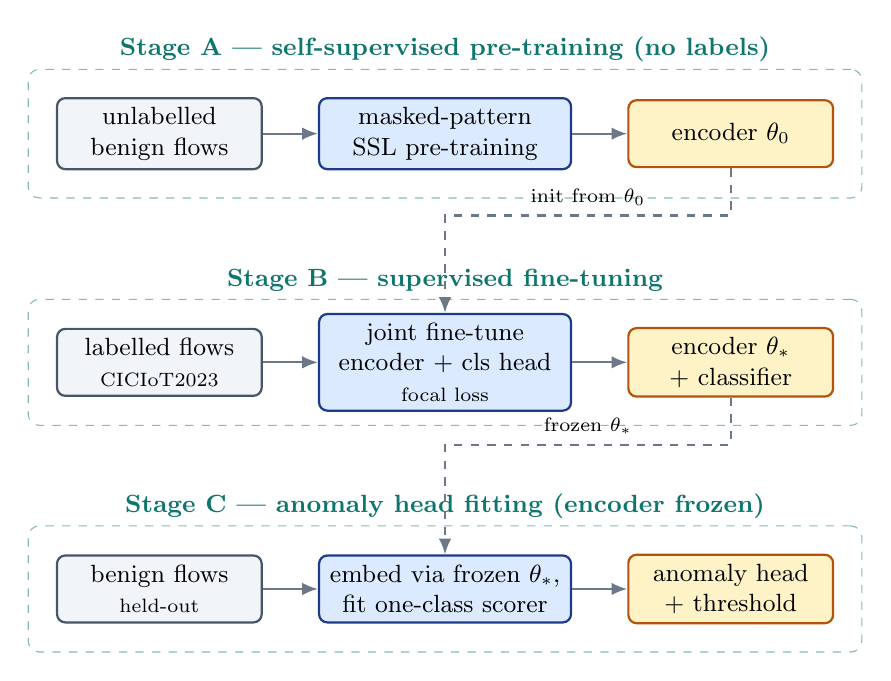
\begin{tikzpicture}[node distance=0.55cm and 0.7cm]

  % Stage A
  \node[data, minimum width=2.6cm] (a1) {unlabelled \\ benign flows};
  \node[proc, right=of a1, minimum width=3.2cm] (a2)
       {masked-pattern \\ SSL pre-training};
  \node[artifact, right=of a2, minimum width=2.6cm] (a3)
       {encoder $\theta_0$};
  \node[draw=accent!50, dashed, rounded corners, fit=(a1)(a3), inner sep=10pt,
        label={[font=\small\bfseries, accent, above=-1pt]:Stage A --- self-supervised pre-training (no labels)}] (sA) {};
  \draw[arr] (a1) -- (a2);
  \draw[arr] (a2) -- (a3);

  % Stage B
  \node[data, minimum width=2.6cm, below=2.0cm of a1] (b1)
       {labelled flows \\ \scriptsize CICIoT2023};
  \node[proc, right=of b1, minimum width=3.2cm] (b2)
       {joint fine-tune \\ encoder + cls head \\ \scriptsize focal loss};
  \node[artifact, right=of b2, minimum width=2.6cm] (b3)
       {encoder $\theta_*$ \\ + classifier};
  \node[draw=accent!50, dashed, rounded corners, fit=(b1)(b3), inner sep=10pt,
        label={[font=\small\bfseries, accent, above=-1pt]:Stage B --- supervised fine-tuning}] (sB) {};
  \draw[arr] (b1) -- (b2);
  \draw[arr] (b2) -- (b3);
  \draw[darr] (a3.south) -- ++(0,-0.6) -| node[pos=0.25, above, font=\scriptsize]{init from $\theta_0$} (b2.north);

  % Stage C
  \node[data, minimum width=2.6cm, below=2.0cm of b1] (c1)
       {benign flows \\ \scriptsize held-out};
  \node[proc, right=of c1, minimum width=3.2cm] (c2)
       {embed via frozen $\theta_*$, \\ fit one-class scorer};
  \node[artifact, right=of c2, minimum width=2.6cm] (c3)
       {anomaly head \\ + threshold};
  \node[draw=accent!50, dashed, rounded corners, fit=(c1)(c3), inner sep=10pt,
        label={[font=\small\bfseries, accent, above=-1pt]:Stage C --- anomaly head fitting (encoder frozen)}] (sC) {};
  \draw[arr] (c1) -- (c2);
  \draw[arr] (c2) -- (c3);
  \draw[darr] (b3.south) -- ++(0,-0.6) -| node[pos=0.25, above, font=\scriptsize]{frozen $\theta_*$} (c2.north);

\end{tikzpicture}
\caption{Training pipeline. Stage A pre-trains the encoder on unlabelled benign flows with a masked-pattern objective; no attack labels are used. Stage B initialises from $\theta_0$ and jointly fine-tunes the encoder and a supervised classification head on labelled CICIoT2023 attack categories, yielding $\theta_*$ and the classifier. Stage C freezes $\theta_*$, embeds a held-out benign set, fits the one-class anomaly scorer (deep SVDD by default) on those embeddings, and calibrates the threshold. At inference (Figure~\ref{fig:inference}), the encoder $\theta_*$ is shared by both heads.}
\label{fig:training}
\end{figure}

\subsection{Stage A --- Self-supervised pre-training}
The Mamba encoder is pre-trained on benign-only CICIoT2023 flows. We use a masked-pattern objective: a random subset of packet positions in the input sequence is masked, and the encoder is trained to predict the masked feature vectors from their context. This is the analogue of masked language modelling, adapted to per-packet features. A contrastive variant over augmented flow views (per ET-SSL) is included as an alternative pre-training objective and ablated. No attack labels are used in this stage. If GPU budget proves the binding constraint, we warm-start from a publicly available Mamba checkpoint and adapt rather than train from scratch.

\subsection{Stage B --- Supervised fine-tuning}
We initialise the encoder from $\theta_0$ and add a two-layer MLP + softmax classification head. The encoder and head are jointly fine-tuned on the labelled CICIoT2023 training set using focal loss. We additionally train a baseline CNN-BiLSTM on aggregated flow statistics in the same stage, so the gain from the flow-pattern + Mamba combination can be cleanly attributed.

\subsection{Stage C --- Anomaly head fitting}
We freeze the fine-tuned encoder $\theta_*$, embed a held-out benign validation set, and fit a one-class scorer on those embeddings. Deep SVDD is the default; Mahalanobis is the fallback. The threshold is calibrated at the 99th percentile of benign validation scores. The held-out benign set is disjoint from the supervised training set.

\subsection{Validation of zero-day capability}
Because the anomaly head is trained without seeing any attack data, we cannot evaluate it by simple held-out test split. We instead evaluate it on \emph{attack classes that were held out from supervised training} --- a leave-one-class-out protocol. The anomaly head's detection rate on these unseen classes is our zero-day proxy.

\subsection{Progressive learning --- absorbing new attack types}
The three-stage training pipeline is also designed to make ongoing updates cheap. When a previously unseen attack type appears in the wild, the system handles it in four steps without retraining from scratch:
\begin{enumerate}[leftmargin=*, itemsep=2pt]
  \item \textbf{Day-zero detection by the anomaly head.} The one-class scorer flags the novel attack as anomalous because it does not look like benign traffic. The analyst sees the alert and the accompanying SHAP attributions.
  \item \textbf{Labelling.} The SOC confirms a sample of flagged flows as attack instances and assigns a new class label.
  \item \textbf{Head-only fine-tuning.} The classifier head is extended with the new class (one additional softmax output) and re-fine-tuned on the new labelled data with a brief replay buffer of the original classes to prevent catastrophic forgetting. The Mamba encoder $\theta_*$ remains \emph{frozen} during this update. This is a small training run --- typically minutes on a single GPU --- because only the lightweight classification head changes.
  \item \textbf{Optional anomaly recalibration.} If the new attack distribution shifts the benign-vs-attack boundary in the projected anomaly space, the SVDD threshold is recalibrated on a fresh benign validation set. The encoder and projection stay fixed.
\end{enumerate}
Full encoder retraining is only required if the \emph{benign} traffic distribution itself shifts (new device classes deployed, network re-architecture, etc.) --- a much rarer event than new-attack arrival. This decoupling of "what's normal" (encoder, expensive to retrain) from "what's malicious" (heads, cheap to update) is the operational payoff of the shared-encoder design.

% =======================================================================
\section{Evaluation Plan}

\subsection{Datasets}
\textbf{CICIoT2023} (primary): supervised training, primary test, and benign pre-training corpus. 105 real devices, 33 attack types, 7 categories. \textbf{TON\_IoT}: cross-dataset generalisation target, never seen during training. \textbf{IoT-23}: real-world malware capture (Mirai, Torii, Okiru, etc.), used as a malware-specific zero-day check.

\subsection{Baselines and what each one quantifies}
\begin{itemize}[leftmargin=*, itemsep=2pt]
  \item \textbf{ET-BERT} (reference upper bound). Quantifies how much accuracy the Mamba detector retains relative to the transformer-class reference at gateway-prohibitive cost. Either run directly on a subset or use published numbers.
  \item \textbf{CNN-BiLSTM on aggregated statistics} (representation control). Isolates the gain from flow-pattern input + Mamba over the conventional aggregated-statistic + sequence-model pipeline.
  \item \textbf{XGBoost on aggregated statistics} (the classical-floor challenge). In the IDS literature, gradient-boosted trees on hand-crafted flow features are routinely competitive with --- and sometimes beat --- deep models on in-distribution test sets. We keep XGBoost as an explicit baseline precisely to answer the ``do we need deep learning at all?'' question. The deep model only earns its complexity if it outperforms XGBoost on the metrics XGBoost \emph{cannot} target: zero-day detection (XGBoost is supervised-only), cross-dataset transfer (the pre-trained encoder is the bet for better transfer), and adversarial robustness. If XGBoost matches our detector on CICIoT2023 in-distribution alone, we report that as a finding, not a failure.
  \item \textbf{Isolation Forest} on aggregated statistics (classical unsupervised baseline). Establishes a non-deep zero-day floor against which the anomaly head must improve.
\end{itemize}

\subsection{Metrics}
Per-class precision, recall, F1; ROC-AUC; PR-AUC (the more honest metric under heavy class imbalance); inference latency at p50, p95, p99; model size in MB post-quantisation. Pre-training is monitored separately via masked-prediction accuracy and contrastive loss curves.

\subsection{Adversarial robustness}
FGSM perturbations on the per-packet feature sequence, constrained to remain in valid feature ranges (we do not allow physically impossible perturbations such as negative packet sizes). We sweep perturbation magnitude $\varepsilon$ and report the detection-rate degradation curve for both heads. Following the recent IoT-IDS adversarial-robustness work~\cite{AdvIoT}, we also test whether SHAP attribution fingerprints reliably separate clean and adversarial inputs --- a practical secondary defence.

\subsection{Edge benchmark}
After supervised training, the encoder and classifier are quantised to int8 (post-training quantisation, no fine-tuning required). We measure inference latency and peak memory on a Raspberry Pi 4 (target hardware to be confirmed with the mentor). Sub-10\,ms p95 per-flow inference is the published edge target and our acceptance criterion.

% =======================================================================
\section{Project Plan}

\subsection{Twelve-week timeline}
\begin{center}
\begin{tabularx}{\linewidth}{@{}lX@{}}
\toprule
\textbf{Week} & \textbf{Milestone} \\
\midrule
1--2  & Environment setup; download and validate CICIoT2023, TON\_IoT, IoT-23; reproduce one published number on each as sanity check. \\
3     & Flow-pattern extraction pipeline (pcap $\to$ per-packet sequence); classical baselines (Isolation Forest, XGBoost) on aggregated statistics. \\
4--5  & \textbf{Stage A} --- self-supervised pre-training of the Mamba encoder on benign CICIoT2023; ablate $K$, encoder depth, masked-fraction. \\
6     & \textbf{Stage B} --- supervised fine-tuning of encoder + classifier head; bring up CNN-BiLSTM baseline on aggregated statistics; bring up ET-BERT comparison. \\
7     & \textbf{Stage C} --- one-class anomaly head fitting; threshold calibration; held-out-class zero-day evaluation. \\
8     & Cross-dataset evaluation on TON\_IoT and IoT-23. \\
9     & SHAP integration on flagged alerts; qualitative case studies on true- and false-positive examples. \\
10    & FGSM adversarial study against both heads; SHAP-fingerprint adversarial-detection check. \\
11    & Post-training int8 quantisation; latency / memory benchmark on gateway hardware. \\
12    & One stretch extension (if time); final report; DRDO presentation. \\
\bottomrule
\end{tabularx}
\end{center}

\subsection{Deliverables}
\begin{enumerate}[leftmargin=*, itemsep=2pt]
  \item Reproducible code repository covering the full pipeline (flow-pattern extraction, pre-training, fine-tuning, anomaly head, evaluation, SHAP, FGSM, quantisation).
  \item Pre-trained Mamba encoder checkpoint $\theta_*$ released alongside the report.
  \item Benchmark table: Mamba detector vs.\ ET-BERT vs.\ CNN-BiLSTM vs.\ Isolation Forest vs.\ XGBoost, across CICIoT2023, TON\_IoT, IoT-23.
  \item Adversarial-robustness study: detection rate vs.\ $\varepsilon$ curves for both heads.
  \item Latency and memory profile of the quantised model on gateway hardware, in tabular form.
  \item Technical report ($\approx$25--30 pages) and a DRDO-presented summary.
\end{enumerate}

\subsection{Risks and mitigations}
\begin{itemize}[leftmargin=*, itemsep=2pt]
  \item \textbf{Pre-training compute budget.} A from-scratch Mamba pre-training run may exceed available GPU time. \emph{Mitigation:} small encoder configuration; restricted pre-training corpus; warm-start from a public Mamba checkpoint if needed.
  \item \textbf{Class imbalance hiding minority-class failure.} \emph{Mitigation:} focal loss; always report per-class precision/recall/F1 alongside aggregate metrics.
  \item \textbf{Cross-dataset degradation}, the standard caveat in IDS literature. \emph{Mitigation:} report honestly, measure rather than target; do not over-claim.
  \item \textbf{Gateway memory overrun.} \emph{Mitigation:} post-training int8 quantisation; fallback to a smaller Mamba configuration; reduce $K$ as last resort.
  \item \textbf{Byte-level adversarial sensitivity.} Byte-level input is known to be more perturbation-sensitive than aggregated statistics. \emph{Mitigation:} the FGSM study is designed to surface and quantify this, not hide it; SHAP-fingerprint defence is the secondary signal.
  \item \textbf{Label noise in CICIoT2023}, documented in follow-up analyses. \emph{Mitigation:} spot-check a sample of training examples manually; report any patterns we find.
\end{itemize}

\subsection{Stretch goals}
\begin{enumerate}[leftmargin=*, itemsep=2pt]
  \item \textbf{Mamba-2 / SSD backbone swap.} If Mamba-1 leaves latency / memory headroom at the gateway, upgrade to Mamba-2 for higher-quality representations at comparable cost.
  \item \textbf{Graph-aware branch (E-GraphSAGE).} Add a third head operating on a per-window device-communication graph; static-per-window graph keeps the branch within edge budget.
  \item \textbf{Federated pre-training.} Distributed pre-training across multiple DRDO sensor sites that cannot share raw pcaps, using FedAvg-style aggregation of the masked-pattern objective.
\end{enumerate}

% =======================================================================
\section*{References}

\begin{thebibliography}{99}

\bibitem{ETBERT} Lin, X., Xiong, G., Gou, G., Li, Z., Shi, J., Yu, J. (2022). ET-BERT: A Contextualized Datagram Representation with Pre-training Transformers for Encrypted Traffic Classification. \emph{Proc.\ WWW '22}. \href{https://arxiv.org/abs/2202.06335}{arxiv.org/abs/2202.06335}

\bibitem{NetMamba} Wang, T., \emph{et al.} (2024). NetMamba: Efficient Network Traffic Classification via Pre-training Unidirectional Mamba. \emph{arXiv:2405.11449}. \href{https://arxiv.org/abs/2405.11449}{arxiv.org/abs/2405.11449}

\bibitem{ETSSL} Anomaly Detection in Encrypted Network Traffic Using Self-Supervised Learning (2025). \emph{Scientific Reports}, Nature. \href{https://www.nature.com/articles/s41598-025-08568-0}{nature.com/articles/s41598-025-08568-0}

\bibitem{S4D} Gu, A., Goel, K., R\'e, C. (2022). On the Parameterization and Initialization of Diagonal State Space Models. \emph{NeurIPS}. \href{https://arxiv.org/abs/2206.11893}{arxiv.org/abs/2206.11893}

\bibitem{Mamba} Gu, A., Dao, T. (2023). Mamba: Linear-Time Sequence Modeling with Selective State Spaces. \emph{arXiv:2312.00752}. \href{https://arxiv.org/abs/2312.00752}{arxiv.org/abs/2312.00752}

\bibitem{SSD} Dao, T., Gu, A. (2024). Transformers are SSMs: Generalized Models and Efficient Algorithms Through Structured State-Space Duality. \emph{ICML}. \href{https://arxiv.org/abs/2405.21060}{arxiv.org/abs/2405.21060}

\bibitem{CICIoT2023} Neto, E.C.P., \emph{et al.} (2023). CICIoT2023: A Real-Time Dataset and Benchmark for Large-Scale Attacks in IoT Environment. \emph{Sensors}, 23(13):5941, MDPI. \href{https://www.mdpi.com/1424-8220/23/13/5941}{mdpi.com/1424-8220/23/13/5941}

\bibitem{Morshedi2025} Morshedi, M., \emph{et al.} (2025). A Comprehensive Review of Deep Learning Techniques for Anomaly Detection in IoT Networks. \emph{Engineering Reports}, Wiley. \href{https://onlinelibrary.wiley.com/doi/full/10.1002/eng2.70415}{onlinelibrary.wiley.com/doi/full/10.1002/eng2.70415}

\bibitem{Sensors2023} A Survey of AI-Based Anomaly Detection in IoT and Sensor Networks (2023). \emph{Sensors}, 23(3):1352, MDPI. \href{https://www.mdpi.com/1424-8220/23/3/1352}{mdpi.com/1424-8220/23/3/1352}

\bibitem{TransformerIoT} Evaluating Large Transformer Models for Anomaly Detection of Resource-Constrained IoT Devices (2025). \emph{Scientific Reports}, Nature. \href{https://www.nature.com/articles/s41598-025-21826-5}{nature.com/articles/s41598-025-21826-5}

\bibitem{XAI} Explainable AI for Zero-Day Attack Detection in IoT Networks (2025). \emph{Discover Internet of Things}, Springer. \href{https://link.springer.com/article/10.1007/s43926-025-00184-8}{doi:10.1007/s43926-025-00184-8}

\bibitem{AdvIoT} Enhancing Adversarial Robustness of IoT IDS (2025). \emph{arXiv:2511.06197}. \href{https://www.arxiv.org/pdf/2511.06197}{arxiv.org/abs/2511.06197}

\bibitem{EGraphSAGE} Lo, W.W., \emph{et al.} E-GraphSAGE: A Graph Neural Network Based Intrusion Detection System for IoT. \emph{arXiv:2103.16329}. \href{https://arxiv.org/pdf/2103.16329}{arxiv.org/abs/2103.16329}

\bibitem{FLIDS} Hybrid DL--Federated Learning Powered IDS for IoT/5G Edge (2025). \emph{arXiv:2509.15555}. \href{https://arxiv.org/html/2509.15555v1}{arxiv.org/abs/2509.15555}

\bibitem{PEIoTDS} Federated Learning for Intrusion Detection in IoT Environments (2025). \emph{Discover Internet of Things}, Springer. \href{https://link.springer.com/article/10.1007/s43926-025-00169-7}{doi:10.1007/s43926-025-00169-7}

\end{thebibliography}

\end{document}
